\documentclass[11pt]{article}
%this is for cyrillic text
\usepackage[main=russian,english]{babel}
%this is needed for changing font
\usepackage{fontspec}
\usepackage[a4paper, top=1cm]{geometry}
%without this double integral \iint doesnt work
\usepackage{mathtools}
\usepackage{physics}
%Чтобы LaTeX-овские лигатуры работали, типа тире, кавычек и прочего
\newfontfamily\cyrillicfont[Mapping=tex-text]{Times New Roman}
\usepackage{pgfplots}
\pgfplotsset{compat=1.8}
%this font has cyrillic letters
\setmainfont{Times New Roman}
\begin{document} 
\pagestyle{empty}

\textbf{5.} Найти циркуляцию векторного поля $\vec{a}$ по контуру $l$ , получающемуся при пересечении заданной плоскости $\alpha$ координатными плоскостями.
\[\vec{a} = \vec{i} + y\vec{j} - zx\vec{k}; \quad \alpha: x + y + 3z = - 3\]
\[(x \leq 0; y \leq 0; z \leq 0).\]
Вычислим Ц по контуру $l (ABCA)$ через криволинейный интеграл первого рода. \\
\begin{center}
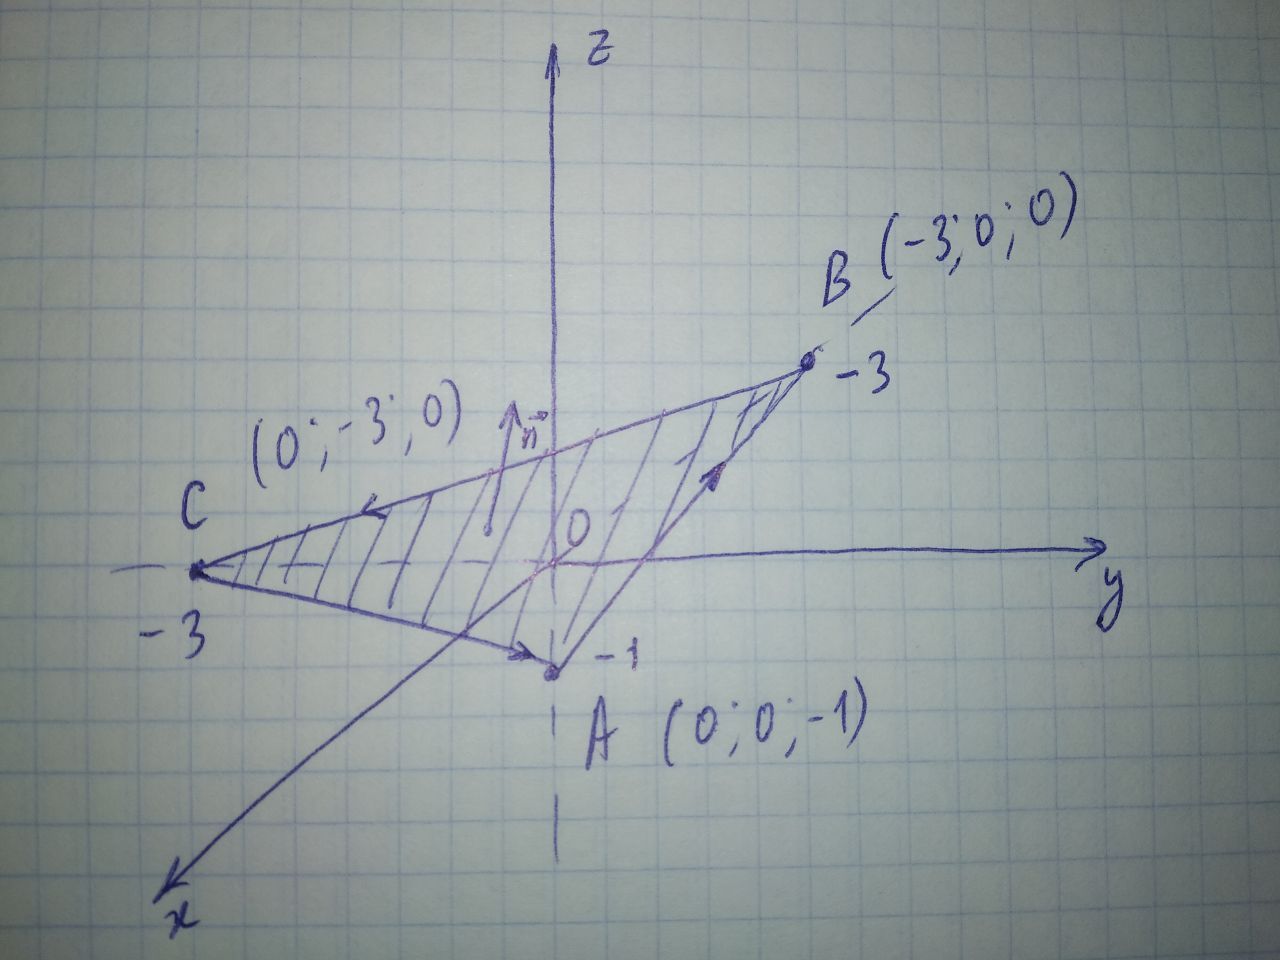
\includegraphics[scale=0.2]{5.jpg} 
\end{center}
По условию $a_x = 1; \quad a_y = y; \quad a_z = -zx$, имеем
\[\text{Ц} = \int_{ABCA}(cos\alpha + ycos\beta - zxcos\gamma)dS\]
С учётом св-ва аддитивности криволинейного интеграла 1 рода по контуру имеем \[\text{Ц} = \Big\lbrace \int_{AB} + \int_{BC} + \int{CA} \Big\rbrace [cos\alpha + y cos\beta - xzcos\gamma]dS \]
\[I_1 = \int_{AB}(cos\alpha + y cos\beta - xzcos\gamma)dS\]
- это интеграл вдоль отрезка $AB$, касательный вектор к которому $\vec{r}$, очевидно, можно взять просто равным вектору $\vec{AB} (-3; 0; 1)$\\
Касательный вектор постоянен, т.к. $AB$ - отрезок прямой. Направляющие косинусы этого вектора совпадают с искомыми $cos\alpha, cos\beta, cos\gamma$
\[cos\alpha = \frac{a_x}{|a|} = \frac{-3}{\sqrt{10}} \quad cos\beta = 0; \quad cos\gamma = \frac{1}{\sqrt{10}}\]
Чтобы вычислить дифференциал дуги $dS$, напишем параметрические уравнения линии $AB$ (как отрезка прямой с направляющим вектором $\vec{r} = \vec{AB}$ и проходящей через точку $A(0; 0; -1)$.
\[
\begin{cases}
	x(t) = 0 - 3t \\
	y(t) = 0 \quad\quad , \quad t\in [0; 1] \\
	z(t) = -1 + t
\end{cases}
\]
Учитывая параметрическое представление линии $AB$ и формулу для вычисления $dS$, получаем
\[dS = \sqrt{(x_t')^2 + (y_t')^2 + (z_t ')^2}dt = \sqrt{(-3)^2 + 1^2} = \sqrt{10}dt\]
Подставляя полученные результаты в равенство для $I_1$, имеем следующее выражение криволинейного интеграла 1го рода $I_1$ через определённый интеграл:
\[I_1 = \int_0^1(-\frac{3}{\sqrt{10}} + 0 \cdot 0 + \frac{1 \cdot(-3t)(t-1)}{\sqrt{10}})\sqrt{10}dt = \]
\[= \int_0^1 (-3 + 3t - 3t^2)dt = -3\int_0^1(t^2 - t + 1)dt =\]
\[= -3(\frac{t^3}{3} - \frac{t^2}{2} + t)\Big|_0^1 = -3 (\frac{1}{3} - \frac{1}{2} + 1) = -3.5\]
Аналогично для $I_2 = \int_{BC}(cos\alpha + y cos\beta - xzcos\gamma)dS$
Имеем 
\[\vec{r} = \vec{BC} = (3; -3; 0); \quad cos\alpha = \frac{1}{\sqrt{2}}; \quad cos\beta = \frac{-3}{3\sqrt{2}} = -\frac{1}{\sqrt{2}}; \quad cos\gamma = 0;\]
Параметрическое представление отрезка
\[
\begin{cases}
	x(t) = -3 + 3t \\
	y(t) = 0 - 3t \quad\quad , \quad t\in [0; 1] \\
	z(t) = 0
\end{cases}
\]
а выражение для $dS$ имеет вид
\[\sqrt{3^2 + (-3)^2}dt = \sqrt{18} = 3\sqrt{2}, \text{Поэтому}\]
\[I_2 = \int_0^1 (\frac{1}{\sqrt{2}}+ -3t\cdot(-\frac{1}{\sqrt{2}})- 0\cdot(3t - 3)\cdot 0)3\sqrt{2}dt = \]
\[= 3\int_0^1(1 + 3t)dt = 3\eval{(t + 3\frac{t^2}{2})}_0^1 = \]\[3(1 + \frac{3}{2}) = 3 + \frac{9}{2} = 4.5 + 3  = 7.5\]
Для $I_3 = \int_{CA}(cos\alpha + y cos\beta - xzcos\gamma)dS$ Получаем \[\vec{r} = \vec{CA} = (0;3;-1); \quad cos\alpha = 0; cos\beta = \frac{3}{\sqrt{10}}; \quad cos\gamma = \frac{-1}{\sqrt{10}}\]
Параметрическое представление отрезка
\[
\begin{cases}
	x(t) = 0 + 0t \\
	y(t) = -3 + 3t \quad\quad , \quad t\in [0; 1] \\
	z(t) = 0 - t
\end{cases}
\]
а выражение для $dS$ имеет вид
\[dS = \sqrt{3^2 + (-1)^2}dt = \sqrt{10}dt\]
\[I_3 = \int_0^1\Big(0 + (3t-3)\frac{3}{\sqrt{10}} - 0\cdot(-t)\big(-\frac{1}{\sqrt{10}}\big)\Big)\sqrt{10}dt = \]
\[= 9\int_0^1(t-1)dt = 9\eval{(\frac{t^2}{2} - t)}_0^1 = 9(\frac{1}{2} - 1) = -4.5\]
\[\text{Ц} = I_1 + I_2 + I_3 = -3.5 + 7.5 - 4.5 = -0.5\]

Вычислим теперь циркуляцию векторного поля $\vec{a}$ с помощью криволинейного интеграла второго рода:
\[\text{Ц} = \int_l a_xdx + a_ydy + a_zdz = \int_{ABCA}dx+ ydy - zxdz\]
Пользуясь аддитивностью
\[\text{Ц} = \Big\lbrace \int_{AB} + \int_{BC} + \int{CA} \Big\rbrace (dx + ydy - zxdz)\]
Разобьём правую часть на 3 слагаемых
\[J_1 = \int_{AB}dx + ydy - zxdz\]
\[
\begin{cases}
	x(t) = 0 - 3t \\
	y(t) = 0 \quad\quad , \quad t\in [0; 1] \\
	z(t) = -1 + t
\end{cases}
\]
Тогда $dx = -3dt; \quad dy = 0; \quad dz = dt$. Поставляя в равенство для $J_1$
\[J_1 = \int_0^1(-3 - (t-1\cdot(-3t))dt = \]
\[= \int_0^1(-3 - (3t - 3t^2))dt = 3\int_0^1(t^2 - t - 1)dt = 3\eval{(\frac{t^3}{3}- \frac{t^2}{2} - t)}_0^1 = \]
\[= 3 (\frac{1}{3} - \frac{1}{2} - 1) = 1 - \frac{3}{2} - 3 = -3.5\]
Аналогично $J_2 = \int_{BC}dx + ydy - xzdz$.
\[
\begin{cases}
	x(t) = -3 + 3t \\
	y(t) = 0 - 3t \quad\quad , \quad t\in [0; 1] \\
	z(t) = 0
\end{cases}
\]
\[dx = 3dt; \quad dy = -3dt; \quad dz = 0; \]
Поэтому
\[J_2 = \int_0^1(3 - 3t(-3)) dt = \int_0^1(3 + 9t)dt = \]
\[= 3\int_0^1(3t + 1)dt = 3\eval{(\frac{3t^2}{2} + t)}_0^1 = 3(\frac{3}{2} + 1) = 4.5 + 3 = 7.5\]
Для $J_3 = \int_{CA}dx + ydy - zxdz$ c учётом
\[
\begin{cases}
	x(t) = 0 + 0t \\
	y(t) = -3 + 3t \quad\quad , \quad t\in [0; 1] \\
	z(t) = 0 - t
\end{cases}
\]
\[dx = 0; \quad dy = 3dt; \quad	dz = -dt \].
\[J_3 = \int_0^1(3t-3)\cdot 3 dt = 9\int_0^1 (t-1)dt = 9\eval{(\frac{t^2}{2} - t)}_0^1 = \]
\[= 9(\frac{1}{2} - 1) = -4.5\]
\[\text{Ц} = J_1 + J_2 + J_3 = -3.5 + 7.5 - 4.5 = -0.5\]

Проверим циркуляцию с помощью формулы Стокса. Вначале вычислим $rot\vec{a}$: \[rot \vec{a} = \begin{vmatrix}
       \vec{i} & \vec{j} & \vec{k}  \\
       \pdv{x} & \pdv{y} & \pdv{z}  \\
       1       & y 		 & -xz
     \end{vmatrix} = \]
\[\vec{i}\Big(-\pdv{(xz)}{y} - \pdv{y}{z}\Big) + \vec{j}\Big(\pdv{(1)}{z} + \pdv{(xz)}{x}\Big) + \vec{k}\Big(\pdv{y}{x}- \pdv{(1)}{y}\Big) = \vec{i}(0) + \vec{j}(z) + \vec{k}\cdot 0 = z\vec{j}\]
\[\text{Ц} = \iint_{\sigma}(0\cdot cos\lambda + zcos\mu + 0\cdot cos\nu)d\sigma \]
- выражение для циркуляции через поверхностный интеграл 1го рода, $\sigma$ - треугольник $ABC$, ограниченный контуром $l$ - ломаной $ABCA$. Итак \\
\[\text{Ц} = \int_\sigma z cos\mu d\sigma\]
Вычислим $cos\mu$.\\
Для этого заметим, что нормаль. к поверхности $\sigma$ (части плоскости $\alpha: x + y + 3z = - 3$) может служить вектор $\vec{n} = (1;1;3)$.
Отметим, что поскольку поверхность $\sigma$ - часть плоскости, то $\vec{n} = const$. Направляющие  косинусы $\vec{n}$ равны
\[cos\lambda = \frac{1}{\sqrt{11}}; \quad cos\mu = \frac{1}{\sqrt{11}}; \quad cos\nu = \frac{3}{\sqrt{11}} \]
Направление вектора $\vec{n}$ совпадает с направлением нормали, согласованной с направлением обхода контура $l$. Поэтому
\[\text{Ц} = \iint_\sigma z\cdot\frac{1}{\sqrt{11}}d\sigma\]
Используя выражение поверхностного интеграла через двойной интеграл по области $D_{yz}$ - проекции $\triangle ABC$ на плоскость $xOz$
\[\text{Ц} = \iint_{D_{xz}} z\frac{1}{\sqrt{11}}\sqrt{(\pdv{y}{x})^2 + 1 + (\pdv{y}{z})^2}dxdz\]
\[y = 3z - x - 3\]
\[\pdv{y}{x} = -1; \quad \pdv{y}{z} = 3\]
\[\sqrt{(\pdv{y}{x})^2 + 1 + (\pdv{y}{z})^2} = \sqrt{1 + 1 + 9} = \sqrt{11}\]
\[\text{Ц} = \iint_{D_{xz}} z\frac{1}{\sqrt{11}}\sqrt{11}dxdz = \iint_{D_{xz}}zdxdz \]
Область интегрирования $D_{xz}$ - это треугольник  $AOB$
\begin{center}
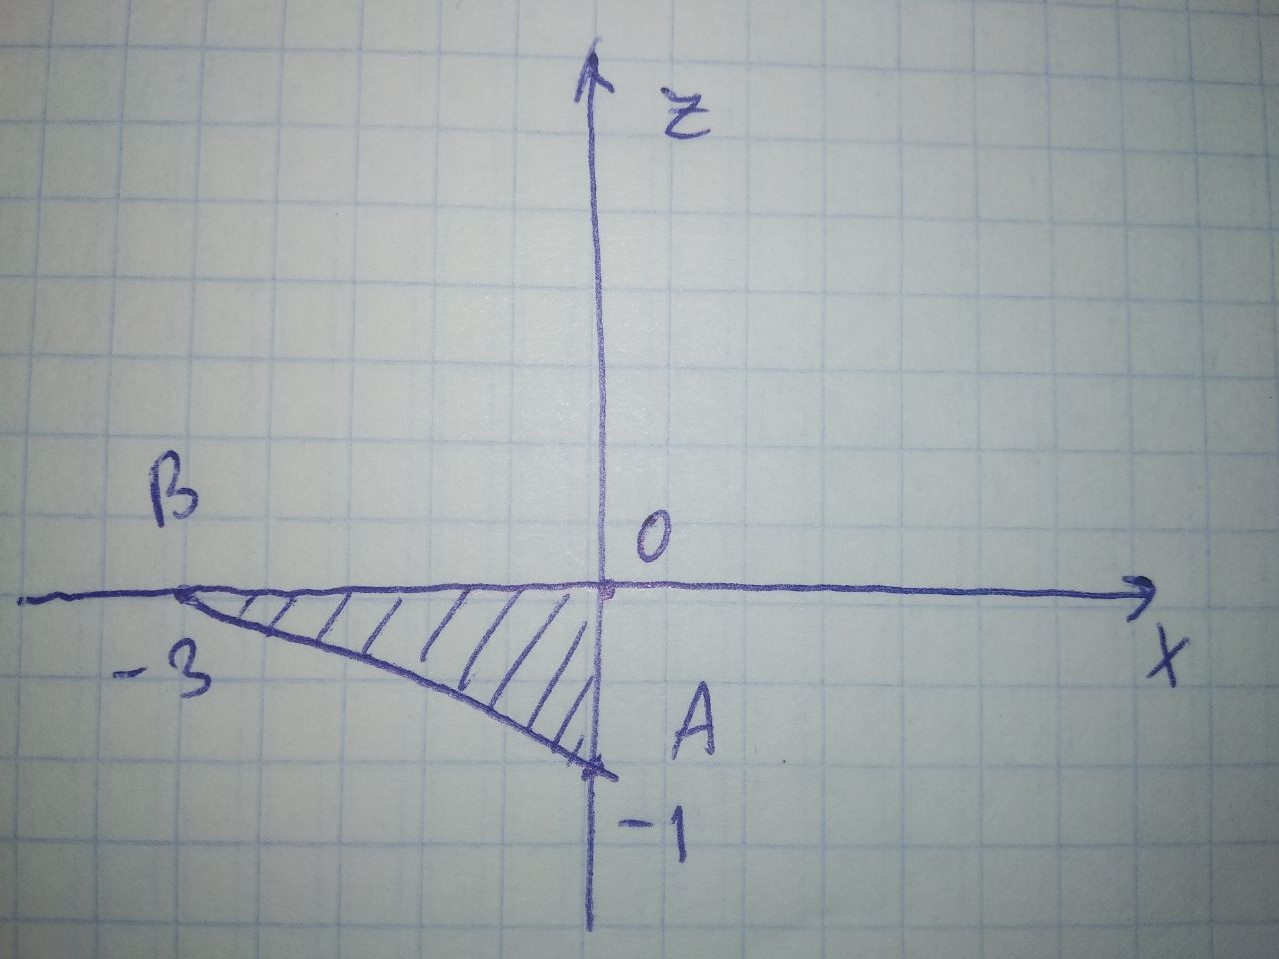
\includegraphics[scale=0.2]{5-stocks.jpg} 
\end{center}
Уравнение прямой имеет вид $z = -1 - \frac{1}{3}x$
\[\text{Ц} = \iint_{D_{xz}}zdxdz = \int_{-3}^0dx\int_{-1-\frac{1}{3}x}^0zdz = \]
\[ =\int_{-3}^0dx\eval{(\frac{z^2}{2})}_{-1-\frac{1}{3}x}^0 = \int_{-3}^0(-\frac{1 + \frac{2}{3}x + \frac{1}{9}x^2}{2})dx = \]
\[= -\frac{1}{2}\eval{(x + \frac{x^2}{3} + \frac{x^3}{27})}_{-3}^0 = -\frac{1}{2}(-(-3 + \frac{9}{3} - \frac{27}{27})) = -\frac{1}{2}\cdot 1 = -0.5\]
Выполним расчёт циркуляции по формуле Стокса, используя при этом поверхностный интеграл 2го рода
\[\text{Ц} = \iint_\sigma (0\cdot dydz + zdxdz + 0\cdot dxdy) = \iint_\sigma zdxdz\]
Выражаем через двойной интеграл, имеем:
\[\text{Ц} = \iint_{D_{xz}} zdxdz\]
Очевидно, что этот интеграл совпадает с соответствующим выражением поверхностного интеграла 1го рода $\iint_\sigma z\frac{1}{\sqrt{11}}d\sigma$ через двойной интеграл. Поэтому
\[\text{Ц} = \iint_{D_{xz}}zdxdz = - 0.5\]\\
\textbf{Ответ:} -0.5
\end{document}

